\section{init} \label{sec-Commands-init}
\index{init}

Defines the simulation cell sizes and the material specification to be used.

\begin{figure}
\begin{center}
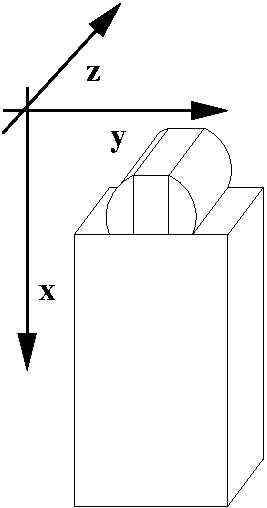
\includegraphics{images/axes}
\caption{Definition of axes in MMonCa}
\end{center}
\label{fig:axes}
\end{figure}

\subsection{Uniform mesh specified using minimum and maximum}

\begin{description}
\item [material=$<$procedure$>$] Specifies the name of a procedure where \MMonCa{} will obtain the material information. The procedure has three input arguments, x, y and z, and returns the name of a valid material.
\item [maxx=$<$X$>$] Maximum X size, in nanometers. (X is depth, see Fig.~\ref{fig:axes})
\item [maxy=$<$Y$>$] Maximum Y size, in nm. Y is width.
\item [maxz=$<$Z$>$] Maximum Z size, in nm.
\item [minx=$<$x$>$] Minimum x size.
\item [miny=$<$y$>$] Minimum y size.
\item [minz=$<$z$>$] Minimum z size.
\item [totalseconds=$<$seconds$>$] Batch execution systems like SLURM require an upper runtime to be specified for the job. Exceeding this limit immediately terminates the job. \MMonCa\ runtimes are hard to estimate in advance. By setting the total \MMonCa\ simulation time to a somewhat lower value than the job time limit, results of a long-lasting simulation can be printed after the interrupted annealing. Only annealing has this implementation; other long-lasting calculations need to come.
\end{description}

Here, the mesh subdivision is ruled by configuration parameters \param{MC/Mesh/spacing.*} where * can be x, y, or z. Example:

\begin{lstlisting}
proc material { x y z } {
        if { $x < 0 } { return "Gas" }
        return "Iron"
}
set sizeX  8
set sizeYZ 80
init minx=-2 miny=0 minz=0 maxx=$sizeX maxy=$sizeYZ maxz=$sizeYZ material=material
\end{lstlisting}

\subsection{Nonuniform mesh specified using division plane locations}

\begin{description}
\item [material=$<$procedure$>$] Specifies the name of a procedure where \MMonCa{} will obtain the material information. The procedure has three input arguments, x, y and z, and returns the name of a valid material.
\item [linesx=$<$\{x1 x2 ...\}$>$] A Tcl array of real numbers in strictly increasing order. These define the location of division planes along the X axis, each one plane perpendicular to that axis.
\item [linesy=$<$\{y1 y2 ...\}$>$] Similar description for the Y axis...
\item [linesz=$<$\{z1 z2 ...\}$>$] and the Z axis.
\item [totalseconds=$<$seconds$>$] as above.
\end{description}

Example: the mesh in Fig.\ref{fig-nonuniform-mesh} can be described as

\begin{lstlisting}
proc material { x y z } {
        if { $x < 2 } { return "Gas" }
        return "Iron"
}
init linesx={0 2 3 4 6} linesy={0 0.5 1.5 3.5 6} linesz={0 1 2 3 4 5 6} material=material
\end{lstlisting}

Here, we define 5 planes perpendicular to the X axis, 5 planes for the Y axis and 7 planes for the Z axis. As these planes cut the simulation area into cells, there will be a total of (5-1)(5-1)(7-1)=112 cells. As for the original equidistant division, each cell is assigned a single material, here defined by the Tcl function in the material parameter.

\subsection{Nonuniform mesh and material specified using a JSON file}

It is also possible to load a JSON file containing all the geometrical and material information. This file has explicitelly to include definitions and sizes of all the volumes involved in the simulation; i.e. underlying substrates, specific structures as well as the gas volumes used in CVD chambers, etc. 

\begin{description}
\item [mesh=$<$filename$>$] Specifies the name of the JSON file.
\item [totalseconds=$<$seconds$>$] as above.
\end{description}

The JSON file contains the locations of the division planes along each axis, together with a list of material IDs for each cell defined by the planes. A mapping of material name to ID used in the cell list must also be provided. Here, the material names must correspond to the long material names in MMonCa. In the example below, Gas is on the top (x is the depth coordinate), below it resides Si:

\begin{lstlisting}
init mesh="mesh.json"
\end{lstlisting}

with the JSON file

\begin{lstlisting}
{
  "linesX": [ 0.0, 1.5, 3.0 ],
  "linesY": [ 0.0, 1.4, 3.0 ],
  "linesZ": [ 0.0, 1.4, 2.8, 4.4, 6.0 ],
  "materialIDs": [ 33, 33, 33, 33, 33, 33, 33, 33,  22, 22, 22, 22, 22, 22, 22, 22 ],
  "materialMapping": { 
    "Silicon": 22,
    "Gas": 33 
  } 
}
\end{lstlisting}

The material ID values must be less than 245, and have nothing to do with MMonCa's internal material IDs (which appear in the log). The materialIDs array must have a length of \(cells_X * cells_Y * cells_Z\), where \(C_i = lines_i\) length - 1. This must hold because the lines* arrays specify the division planes for the mesh, and the cells are the areas divided by these planes.

The materialIDs array run first along the Z axis, then on Y and then on X. (x is the depth coordinate) In other words, if we take the index i (starting from 0) of a number in the materialIDs array, the cell indices along the X, Y and Z axes can be calculated by

\begin{lstlisting}
ix = i / cellsY / cellsZ
iy = (i % (cellsY * cellsZ)) / cellsZ
iz = (i % (cellsY * cellsZ)) % cellsZ
\end{lstlisting}
